% !TEX root = ./article.tex

\documentclass{article}

\usepackage{mystyle}
\usepackage{myvars}



%-----------------------------

\begin{document}

	\maketitle % Insert title

	\thispagestyle{fancy} % All pages have headers and footers


%-----------------------------
%	ABSTRACT
%-----------------------------

	\begin{abstract}
		\noindent En este documento se realiza una descripción acerca de la \emph{Regresión Lineal Múltiple} y la \emph{Regresión Logística} desde el punto de vista del ámbito de la \emph{Inteligencia Artificial}. Además, se han realizado implementaciones de dichas técnicas en el lenguaje \emph{Octave}(\emph{MatLab}) para después utilizarlas en la realización de varios experimentos de comparación y cotas de tasa de error con los conjuntos de datos \emph{Housing} \cite{dataset:housing} y \emph{Wine}\cite{dataset:wine}
	\end{abstract}

%-----------------------------
%	TEXT
%-----------------------------


	\section{Introducción}
	\label{sec:introducción}

		\subsection{Regresión Lineal Múltiple}

			\paragraph{}
			La \emph{regresión lineal} es un modelo matemático usado para aproximar la relación de dependencia entre una variable dependiente $Y$, las variables independientes $X_i$ y un término aleatorio $\epsilon$. Este modelo se describe en la ecuación \eqref{eq:linear_regresion} donde las variables $\beta_i$ representan los pesos que ajustan los valores de las variables $X_i$ para aproximar su suma total al valor deseado ( $= Y$ ).

			\begin{equation}
			\label{eq:linear_regresion}
				{\displaystyle Y=\beta _{0}+\beta _{1}X_{1}+\beta _{2}X_{2}+\cdots +\beta _{p}X_{p}+\varepsilon }
			\end{equation}

			\paragraph{}
			Por tanto, en este modelo de aprendizaje, se trata de aprender el valor de dichos pesos a partir de un conjunto de datos de entrenamiento. La estrategia que se ha utilizado en este caso ha sido el ajuste por mínimos cuadrados, el cual trata de minimizar la diferencia global ajustando dichos pesos. Para dicha tarea se ha utilizado la implementación en \emph{Octave} que se muestra en la figura \ref{code:lineal_regression}.

			\begin{figure}[h]
				\centering
				\inputminted{octave}{./code/regresion_lineal_k.m}
				\caption{Octave: /src/regresion\_lineal\_k.m}
				\label{code:lineal_regression}
			\end{figure}


		\subsection{Regresión Logística}

			\paragraph{}
			La estrategia de \emph{Regresión Logística} se corresponde con una transformación de la lineal descrita en la sección anterior. El nombre de dicha técnica viene dado por la función utilizada para la transformación (función logística), que se describe en la ecuación \eqref{eq:logistic_function}. Mediante esta transformación se consigue que los resultados de la regressión (variable $Y$) cambien su dominio al rango $[0,1]$.

			\begin{equation}
			\label{eq:logistic_function}
				f(x)={\frac  {1}{1+{\mathrm  e}^{{-k(x-x_{0})}}}}
			\end{equation}

			\paragraph{}
			El planteaminto de esta estrategia en el campo de la \emph{Inteligencia Artifical} es diferente respecto de la anterior. En este caso en lugar de tratar de aproximar la regresión al valor deseado, se utiliza para conocer el grado de similitud de los datos de entrada respecto de una determinada clase. Por tanto, funciona como un clasificador de carácter binario si se fija el valor de destino cuando la regresión cruza el umbral $0.5$.

			\paragraph{}
			Para extender dicho funcionamiento a clasificadores de varias clases se utiliza una estrategia de clasificación por pares, lo cual conlleva la utilización de $\frac{k(k-1)}{2}$ clasficadores cuando existen $k$ clases distintas de destino. El valor que se asigna es el de la clase que más veces haya resultado ganadora y se toma como un fallo los casos de empate.

			\paragraph{}
			El algoritmo de aprendizaje de pesos utilizado  (al igual que en el caso anterior) se describe mediante su implementación en el lenguaje \emph{Octave} en la figura \ref{code:logistic_regression}. Dicha implementación se refiere al ajuste por mínimos cuadrados al igual que en el caso anterior. En este caso se pueden realizar varias iteraciones para el ajuste, pero se ha comprobado que para el conjunto de datos utilizada una iteración ofrece buenos resultados.

			\begin{figure}[h]
				\centering
				\inputminted{octave}{./code/regresion_logistica_k.m}
				\caption{Octave: /src/regresion\_logistica\_k.m}
				\label{code:logistic_regression}
			\end{figure}



	\section{Evaluación de resultados a partir de distintas cotas de error relativo para Regresión Lineal Múltiple}
	\label{sec:e1}

		\paragraph{}
		En esta sección se realiza un experimento para estudiar la evolución de la tasa de error conforme aumenta la cota de error relativo fijada para admitir una instancia como clasificada de manera correcta. El algoritmo utilizado es el de Regresión Lineal Múltiple mediante el aprendizaje por mínimos cuadrados descrito anteriormente.

		\paragraph{}
		El conjunto de datos que se ha utilizado para dichos experimentos es \textbf{Housing Data Set} \cite{dataset:housing}, que está formado por \textbf{506 instancias}. Dichas instancias contienen \textbf{13 atributos} de carácter númerico. La \textbf{clase de destino es de carácter numérico} (por lo que es una regresión y no una clasificación). En cuanto a la metodología experimental, se ha seguido una extrategia de \textbf{HoldOut} con particionamiento de los datos de manera que $\frac{2}{3}$ son utilizados en la fase de entrenamiento y $\frac{1}{3}$ en la de test.

		\paragraph{}
		Los resultados obtenidos tras los experimentos se muestran de manera tabular en la tabla \ref{table:e1} mientras que se puede apreciar la evolución conforme aumenta el rango de la cota de error de manera gráfica en la figura \ref{plot:e1}.

		\begin{figure}[h]
			\begin{center}
				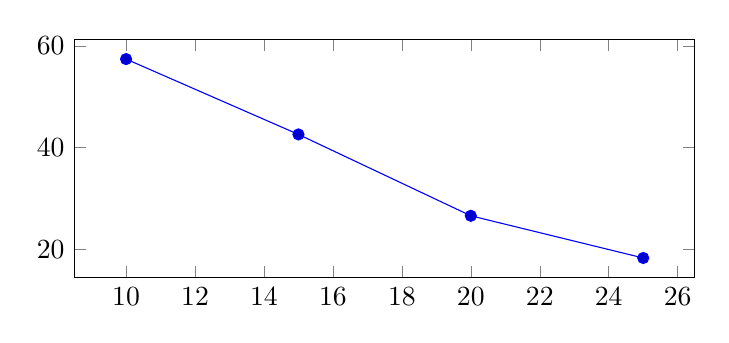
\begin{tikzpicture}
					\begin{axis}[
						% only scale the axis, not the axis including the ticks and labels
						scale only axis=true,
						% set `width' and `height' to the desired values
						width=0.65\textwidth,
						height=0.25\textwidth,
						]
						\addplot coordinates {
							(10,57.396)
							(15,42.604)
							(20,26.627)
							(25,18.343)
						};
					\end{axis}
				\end{tikzpicture}
			\end{center}
			\caption{Evolución de la tasa de error para la \emph{Regresión Lineal Múltiple} sobre el conjunto de datos \emph{Housing} conforme aumenta la cota máxima de error relativo}
			\label{plot:e1}
		\end{figure}

		\begin{table}[h]
			\centering
			\small
			\begin{tabu}{ | c | c | c | c | c | }
				\hline
					& \multicolumn{4}{ c | }{Regresión --- Housing Dataset} \\ \hline
					& \emph{Lineal 10\%} & \emph{Lineal 15\%} & \emph{Lineal 20\%} & \emph{Lineal 25\%}\\ \cline{2-5}
				Error HoldOut						& $57.396\%$	 & $42.604\%$ & $26.627\%$ & $18.343\%$ \\
				\hline
			\end{tabu}
			\caption{Evolución de la tasa de error para la \emph{Regresión Lineal Múltiple} sobre el conjunto de datos \emph{Housing} conforme aumenta la cota máxima de error relativo}
			\label{table:e1}
		\end{table}

	\section{Comparación de resultados entre Regresión Logística y Regresión Lineal Múltiple}
	\label{sec:e2}

		\paragraph{}
		En esta sección se realiza un experimento para estudiar la tasa de error obtenida mediante la estrategia de \emph{Regresión Logística} para después compararla con los resultados obtenidos mediante la estrategia de \emph{Regresión Lineal}. Dicha labor es posible cuando la clase de destino es numérica pero se puede discretizar. (En este caso es de carácter entero y acotada por lo que su discretización es trivial). Puesto que no es de tipo binario es necesario seguir la estrategía de clasificación por pares tal y como se ha descrito anteriormente.

		\paragraph{}
		El conjunto de datos que se ha utilizado para dichos experimentos es \textbf{Wine Data Set} \cite{dataset:wine}, formado por \textbf{178 instancias}. Dichas instancias contienen \textbf{12 atributos} de carácter númerico. La \textbf{clase de destino es de carácter numérico}. Sin embargo, en este caso es de tipo entero, por lo que puede ser vista como una variable categórica. En cuanto a la metodología experimental, se ha seguido una extrategia de \textbf{HoldOut} con particionamiento de los datos de manera que $\frac{2}{3}$ son utilizados en la fase de entrenamiento y $\frac{1}{3}$ en la de test.

		\paragraph{}
		Los resultados obtenidos tras los experimentos se muestran de manera tabular en la tabla \ref{table:e2}. Además, se muestran de manera gráfica en la figura \ref{plot:e2}.


		\begin{figure}[h]
			\begin{center}
				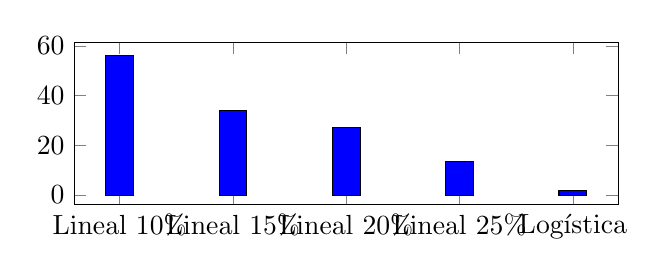
\begin{tikzpicture}
					\begin{axis}[
						symbolic x coords={Lineal 10\%,Lineal 15\%,Lineal 20\%,Lineal 25\%,Logística},
						width=0.7\textwidth,
						height=0.3\textwidth,
						xtick=data]
						\addplot[ybar, fill=blue] coordinates {
							(Lineal 10\%, 55.932)
							(Lineal 15\%, 33.898)
							(Lineal 20\%, 27.119)
							(Lineal 25\%, 13.559)
							(Logística, 1.6949)
						};
					\end{axis}
				\end{tikzpicture}
			\end{center}
			\caption{Resultados obtenidos a nivel de tasa de error mediante \emph{Regresión Lineal Múltiple} y \emph{Regresión Logística} sobre el conjunto de datos \emph{Wine}}
			\label{plot:e2}
		\end{figure}

		\begin{table}[h]
			\centering
			\small
			\begin{tabu}{ | c | c | c | c | c | c | }
				\hline
					& \multicolumn{5}{ c | }{Regresión --- Wine Dataset} \\ \hline
					&\emph{Lineal 10\%} & \emph{Lineal 15\%} & \emph{Lineal 20\%} & \emph{Lineal 25\%} & \emph{Logística}\\ \cline{2-6}
				Error HoldOut	& $55.932\%$	 & $33.898\%$ & $27.119\%$ & $13.559\%$	& $1.6949\%$ \\
				\hline
			\end{tabu}
			\caption{Resultados obtenidos a nivel de tasa de error mediante \emph{Regresión Lineal Múltiple} y \emph{Regresión Logística} sobre el conjunto de datos \emph{Wine}}
			\label{table:e2}
		\end{table}

		\paragraph{}
		Tal y como se puede apreciar tras analizar los resultados, a través de la \emph{Regresión Logística} se obtienen resultados mucho más óptimos. Sin embargo, para aplicar dicha técnica es necesario que la clase de destino esté discretizada. Además conlleva un mayor coste computacional derivado de la estrategia de clasificación por pares, que incrementa en un orden cuadrático los costes conforme aumentan el número de clases de destino.



%-----------------------------
%	Bibliographic references
%-----------------------------
	\nocite{garciparedes:machine-learning-regression}
	\nocite{subject:taa}
  \bibliographystyle{alpha}
  \bibliography{bib/misc}

\end{document}
